% Options for packages loaded elsewhere
\PassOptionsToPackage{unicode}{hyperref}
\PassOptionsToPackage{hyphens}{url}
%
\documentclass[
]{article}
\usepackage{lmodern}
\usepackage{amssymb,amsmath}
\usepackage{ifxetex,ifluatex}
\ifnum 0\ifxetex 1\fi\ifluatex 1\fi=0 % if pdftex
  \usepackage[T1]{fontenc}
  \usepackage[utf8]{inputenc}
  \usepackage{textcomp} % provide euro and other symbols
\else % if luatex or xetex
  \usepackage{unicode-math}
  \defaultfontfeatures{Scale=MatchLowercase}
  \defaultfontfeatures[\rmfamily]{Ligatures=TeX,Scale=1}
\fi
% Use upquote if available, for straight quotes in verbatim environments
\IfFileExists{upquote.sty}{\usepackage{upquote}}{}
\IfFileExists{microtype.sty}{% use microtype if available
  \usepackage[]{microtype}
  \UseMicrotypeSet[protrusion]{basicmath} % disable protrusion for tt fonts
}{}
\makeatletter
\@ifundefined{KOMAClassName}{% if non-KOMA class
  \IfFileExists{parskip.sty}{%
    \usepackage{parskip}
  }{% else
    \setlength{\parindent}{0pt}
    \setlength{\parskip}{6pt plus 2pt minus 1pt}}
}{% if KOMA class
  \KOMAoptions{parskip=half}}
\makeatother
\usepackage{xcolor}
\IfFileExists{xurl.sty}{\usepackage{xurl}}{} % add URL line breaks if available
\IfFileExists{bookmark.sty}{\usepackage{bookmark}}{\usepackage{hyperref}}
\hypersetup{
  pdftitle={Homework 01},
  pdfauthor={Ming Lin},
  hidelinks,
  pdfcreator={LaTeX via pandoc}}
\urlstyle{same} % disable monospaced font for URLs
\usepackage[margin=1in]{geometry}
\usepackage{graphicx}
\makeatletter
\def\maxwidth{\ifdim\Gin@nat@width>\linewidth\linewidth\else\Gin@nat@width\fi}
\def\maxheight{\ifdim\Gin@nat@height>\textheight\textheight\else\Gin@nat@height\fi}
\makeatother
% Scale images if necessary, so that they will not overflow the page
% margins by default, and it is still possible to overwrite the defaults
% using explicit options in \includegraphics[width, height, ...]{}
\setkeys{Gin}{width=\maxwidth,height=\maxheight,keepaspectratio}
% Set default figure placement to htbp
\makeatletter
\def\fps@figure{htbp}
\makeatother
\setlength{\emergencystretch}{3em} % prevent overfull lines
\providecommand{\tightlist}{%
  \setlength{\itemsep}{0pt}\setlength{\parskip}{0pt}}
\setcounter{secnumdepth}{-\maxdimen} % remove section numbering
\ifluatex
  \usepackage{selnolig}  % disable illegal ligatures
\fi

\title{Homework 01}
\author{Ming Lin}
\date{}

\begin{document}
\maketitle

I pledge my honor that I have abided by the Stevens Honor System

Problem 1(i)

\begin{center}\includegraphics{homework01_files/figure-latex/unnamed-chunk-2-1} \end{center}

\begin{center}\includegraphics{homework01_files/figure-latex/unnamed-chunk-2-2} \end{center}

It seems that for the values within x pie chart \textasciitilde50\% of
its values are greater than 2 and less than 4. Whereas y pie chart all
values are distributed evenly.

Problem 1(ii)

\begin{center}\includegraphics[width=0.5\linewidth,height=0.5\textheight]{homework01_files/figure-latex/unnamed-chunk-3-1} \end{center}

\begin{verbatim}
##    Min. 1st Qu.  Median    Mean 3rd Qu.    Max. 
##   0.200   1.275   2.250   2.407   2.900   9.000
\end{verbatim}

\begin{verbatim}
## Warning in if (plot) {: the condition has length > 1 and only the first element
## will be used
\end{verbatim}

\begin{center}\includegraphics[width=0.5\linewidth,height=0.5\textheight]{homework01_files/figure-latex/unnamed-chunk-3-2} \end{center}

Variance{[}X{]}:4.5684066 Outlier{[}X{]}:9

\begin{center}\includegraphics[width=0.5\linewidth,height=0.5\textheight]{homework01_files/figure-latex/unnamed-chunk-4-1} \end{center}

\begin{verbatim}
##    Min. 1st Qu.  Median    Mean 3rd Qu.    Max. 
##   0.100   1.400   5.300   4.879   7.575   9.900
\end{verbatim}

\begin{verbatim}
## Warning in if (plot) {: the condition has length > 1 and only the first element
## will be used
\end{verbatim}

\begin{center}\includegraphics[width=0.5\linewidth,height=0.5\textheight]{homework01_files/figure-latex/unnamed-chunk-4-2} \end{center}

Variance{[}Y{]}: 11.247967 Outlier{[}Y{]}: 0

Problem 1(iii)

\begin{center}\includegraphics[width=0.5\linewidth,height=0.5\textheight]{homework01_files/figure-latex/unnamed-chunk-5-1} \end{center}

Correlation Coefficient:

\begin{verbatim}
## [1] 0.5730545
\end{verbatim}

X and Y have a modern linear association because of their positive
correlation coefficient

Problem 1(iv)

\begin{center}\includegraphics[width=0.5\linewidth,height=0.5\textheight]{homework01_files/figure-latex/unnamed-chunk-7-1} \end{center}

Removed (9.0, 9.8) and changed the correlaton coefficient to 0.4586256.

Problem 1(v)

The main difference observed between the numerical results in part 3 and
4 is that part 3 had a positive relation, while part 4 had a weaker
relation. This change is a result of removing the outlier in part 4.

Problem 1(vi)

\includegraphics[width=0.5\linewidth,height=0.5\textheight]{homework01_files/figure-latex/p1-vi-1}
\includegraphics[width=0.5\linewidth,height=0.5\textheight]{homework01_files/figure-latex/p1-vi-2}

After observing the both QQ plots, it seems that x is more likely to be
of normal distribution.

Problem 2

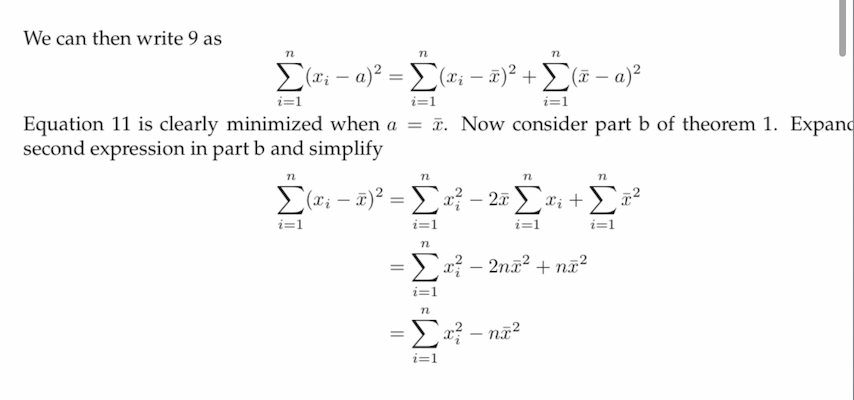
\includegraphics{/Users/minglin/Stevens-IT/MA331/hw01/Problem2.png}

Using the proof above this proves the first part of problem 2 and the
second part becuase 1/n is a constant.

\end{document}
